\documentclass[a4paper, 11pt]{report}
\usepackage[utf8]{inputenc} 
\usepackage[T1]{fontenc}
\usepackage[frenchb]{babel} %ou \usepackage[francais]{babel} 
\usepackage{url} %écrire des adresses cliquables
\usepackage{lmodern} %changer pack de police
\usepackage[top=3cm, bottom=3cm, left=3cm, right=3cm]{geometry} %gérer les marges
\usepackage{color}
\usepackage[babel=true]{csquotes} % csquotes va utiliser la langue définie dans babel
\usepackage{graphicx}
\usepackage[space]{grffile}
\usepackage{listings}
\lstset{language=C,basicstyle=\small,frame=leftline,captionpos=b,linewidth=175mm,breaklines=true, ,identifierstyle=\ttfamily, numbers=none, numberstyle=\tiny, stepnumber=5, numberfirstline=true, showstringspaces=false}
%\input{milstd}
\DeclareGraphicsExtensions{.jpeg, .png , .gif, .bmp}
%\usepackage{eurosym}
\usepackage{array}
\newcolumntype{M}[1]{>{\raggedright}m{#1}}
\usepackage{wrapfig}


%%%%%%%%%%%%%%%%%%%%%%%%%
\begin{document}


% placement des elements
\makeatletter
	\def\clap#1{\hbox to 0pt{\hss #1\hss}}%
	\def\ligne#1{%
	\hbox to \hsize{%
	\vbox{\centering #1}}}%
	\def\haut#1#2#3{%
	\hbox to \hsize{%
	\rlap{\vtop{\raggedright #1}}%
	\hss
	\clap{\vtop{\centering #2}}%
	\hss
	\llap{\vtop{\raggedleft #3}}}}%
	\def\bas#1#2#3{%
	\hbox to \hsize{%
	\rlap{\vbox{\raggedright #1}}%
	\hss
	\clap{\vbox{\centering #2}}%
	\hss
	\llap{\vbox{\raggedleft #3}}}}%
	\def\maketitle{%
	\thispagestyle{empty}\vbox to \vsize{%
	\haut{}{\@blurb}{}
	\vfill
	\vspace{1cm}
\begin{flushleft}
	%\usefont{OT1}{ptm}{m}{n}
	\huge \@title
\end{flushleft}
	\par
	\hrule height 4pt
	\par
\begin{flushright}
	%\usefont{OT1}{phv}{m}{n}
	\Large \@author
	\par
\end{flushright}
	\vspace{1cm}
	\vfill
	\vfill

\begin{center}
	
\includegraphics[width=7cm]{logo_UTBM2.jpg}
\end{center}

\bas{}{Printemps 2013}{}
}%
\cleardoublepage
}
\def\date#1{\def\@date{#1}}
\def\author#1{\def\@author{#1}}
\def\title#1{\def\@title{#1}}
\def\location#1{\def\@location{#1}}
\def\blurb#1{\def\@blurb{#1}}
\date{\today}
\author{}
\title{}

% informations
\location{Belfort}\blurb{}
\makeatother
\title{Rapport de projet - Affectation des fréquences dans les réseaux mobiles}
\author{\small{Thomas Gloriod, Paul Locatelli et Pierre Rognon}}
\blurb{%
	\textbf{AG41 - Optimisation et recherche opérationnelle}\\
	Université de Technologie de Belfort-Montbéliard
}% 


\maketitle
\tableofcontents 
%%%%%%%%

\chapter{Introduction}
Afin de clore l'étude concernant l'optimisation et la recherche opérationnelle, un projet a été proposé. Ce projet concerne l'affectation de fréquences dans le cadre d'antennes pour les réseaux mobiles. L'enjeu réside dans le fait que cette affectation se joue sur un carte qui est familière ici puisque l'on se concentrera sur le Territoire de Belfort.\\
Le problème d'affectation de fréquences est un problème type en recherche opérationnelle. Il est donc connu de tous les initiés de cette discipline.\\
Plus précisément, ce problème s'apparente à un problème de coloration de graphe. Il s'agit ici d'attribuer des fréquences à différents secteurs d'une même zone. La contrainte consiste à éviter le plus possible que deux secteurs limitrophes émettent sur la même fréquence.\\
La modélisation de ce problème représentant un travail important, le projet consiste seulement à se pencher sur la méthode de résolution. Une première partie consiste donc à trouver une solution initiale, c'est-à-dire affecter une première fois les fréquences sans se préoccuper outre mesure de l'efficacité de cette affectation. La seconde partie consiste à améliorer cette affectation en proposant des solutions plus efficaces à l'aide d'un algorithme de notre choix. Ici, le choix s'est porté sur un algorithme de recherche tabou.

\chapter{Présentation du sujet}

	\section{Détails du problème}
	Le département étudié, ici le Territoire de Belfort comporte 36 secteurs, chacun étant divisé en maximum trois secteurs. On obtient ainsi un total de 88 secteurs. Trois fréquences sont disponibles pour chaque secteur. Ces fréquences sont donc numérotées 1, 2 et 3 afin de reconna\^itre facilement celle-ci. \\

\begin{center}
	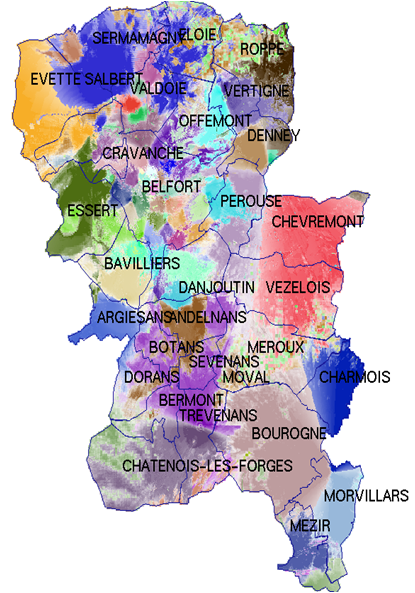
\includegraphics[width=5cm]{carte.png}\\
	\emph{Cette carte représente le territoire qui sera étudié par ce projet soit le département du Territoire de Belfort.\\}
\end{center}

	Chaque secteur reçoit donc dans son affectation  un secteur en fréquence 1, un autre en fréquence 2 et un dernier en fréquence 3. Sur la carte ci-dessous, on peut voir l'agencement théorique de sites entre eux ainsi que la division en secteurs de ceux-ci.
	
	\begin{center}
		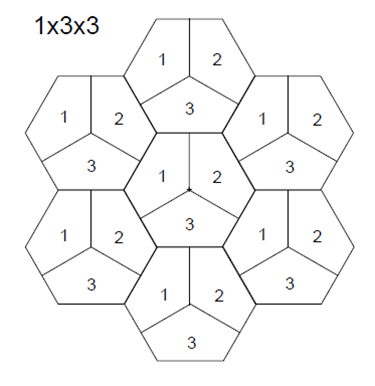
\includegraphics[width=5cm]{ruche}\\
		\emph{Chaque site est délimité en trois secteurs ici identiques mais qui peuvent en réalité varier et ont des frontières plus floues.\\}
	\end{center}

Pour que les clients soient couvert, les secteurs ayant une frontière communes doivent avoir des fréquences différentes afin de minimiser les interférences.\\
Cependant, il n'est pas aisé de savoir si des clients observent des interférences. C'est pourquoi, au sein du territoire, 12 695 points test permettent d'évaluer la qualité de l'allocation des fréquences. Chaque points test est caractérisé par un nombre de clients et le débit souhaité pour chacun. 

	\section{Objectifs}

	L'objectif ici se cache derrière un premier objectif d'ordre technique. En effet, il faut tout d'abord réduire au maximum le nombre de fréquences égales qui se chevaucheraient. Par le chevauchement, on entend une frontière entre deux secteurs, de sites différents, affectés à la même fréquence.\\
	Cependant, derrière cet objectif, le fait de minimiser les conflits, un autre objectif final se cache. Chaque interférence générée par un conflit génère en effet une zone dans laquelle le signal risque fortement d'\^etre perturbé et d’empêcher l'utilisation d'un téléphone par un client potentiel. C'est donc ce problème que l'on cherche à minimiser.


\chapter{Principe de résolution}
	
	La résolution de ce problème peut se faire de deux façons totalement différentes. La première est de manière exacte. L'utilisation de méthode exacte demanderait le calcul de 6\up{36} soit environ 10\up{28} allocation de fréquences différentes. Le temps de calcul n'est donc pas réalisable aujourd'hui, les ordinateurs actuels n'étant pas assez puissants. C'est pourquoi pour ce genre de problème ou le nombre de solution est trop importante, les méthode de résolution approchée sont utilisées.

		\section{Le choix d'une méthode approchée}
		Le principe de cette méthode de résolution est simple. On cherche d'abord une solution au problème, soit de manière aléatoire, soit en en calculant pas trop mauvaise.
		Une liste de voisins à cette solution est ensuite définie. Les voisins sont alors issus de règles précises définies auparavant suivant la méthode approchée à utiliser.
		Il faut ensuite évaluer tous ces voisins afin d'améliorer la solution si possible. La réitération de cette méthode un grand nombre de fois permet de balayer de nombreuses solutions et d'approcher voire de trouver la solution optimale.\\
		L'avantage de ces méthodes approchées est qu'à défaut d'être certain de trouver à coup sûr la bonne solution, il est toujours possible de trouver une solution dont on peut se satisfaire et ce, de manière beaucoup plus rapide que pour une méthode exacte.\\
		Parmi les méthodes approchées, un choix a dû être fait pour ce projet. Ce choix s'est porté sur l'algorithme de la recherche tabou.

		\section{La recherche tabou}
		L'algorithme de recherche tabou permet d'améliorer une simple recherche du meilleur voisin (méthode du hill climbing). En effet, si l'on recherche simplement le meilleur voisin à chaque itération, il est possible quel l'algorithme bloque sur un extremum local. Si la solution n'a que des voisins plus mauvais, l'algorithme va donc considérer que c'est la meilleure solution, même si une solution plus intéressante est disponible.\\
		La recherche tabou permet d'éviter de bloquer dans la plupart des extremums locaux. Cela paraissait donc un choix intéressant dans le cas de l'affectation de fréquences. En effet, le nombre de solution étant relativement important, il est très fortement probable que des extremums locaux existent. L'utilisation de la recherche tabou va éviter de rester bloquer dans un extremum et ainsi d'explorer plus de solutions dans un même nombre d'itérations. Le principe de recherche des voisins de la recherche tabou étant similaire au hill climbing, peu de modifications sont nécessaires. Il suffit, lorsqu'une solution voisine est étudiée, de la placer dans une liste "tabou". On lui attribue alors une durée tabou qui va permettre d'indiquer le nombre d'itérations durant lequel il sera interdit de retourner sur la solution. La liste tabou va donc enregistrer toutes les solutions actuellement interdites ainsi que la durée restante. Dans le cas où une solution présente dans la liste tabou est un extremum local, on évitera ainsi d'y retourner et l'on pourra s'en éloigner.

\chapter{Algorithme développé}

	Comme déjà abordé précédemment, deux partie ont été nécessaires pour pouvoir générer une solution optimale. La première partie consiste à générer une première solution, la seconde à l'améliorer.

	\section{Génération de la solution initiale}
	
	Pour la recherche d'une première solution, la démarche s'est effectuée en plusieurs étapes. La première consistait à lister les méthodes possibles, la seconde à l'implémenter et enfin la dernière à l'évaluer afin de savoir s'il est possible de s'en satisfaire.\\
	La première méthode possible, la plus évidente aussi, est le choix d'une solution aléatoire. Dans ce cas, aléatoire signifie une attribution de la fréquence 1, 2 ou 3 aux secteurs d'un site de façon non redondante, mais sans se préoccuper des autres sites.\\
	Une fois les paramètres de cette méthode choisi, l'algorithme a été implémenté dans le logiciel afin de tester la méthode. Le code de l'algorithme est disponible en annexe 1.\\
	La fonction en annexe est appelée pour chaque sites. Ainsi, à chaque fois, le but est de créer un tableau de taille 3. Chaque case du tableau est remplie par un chiffre, soit 0, soit 1, soit 2. Ces trois chiffres permettent de donner un indice et donc une fréquence à chacun des trois secteurs d'un site.\\
	Pour cela, on va créer deux tableaux, un destiné à être retourné, un autre qui va servir de support. Ce dernier reçoit les trois fréquences à allouer. A chaque fois, on prend aléatoirement une case de ce tableau et on la recopie dans le tableau à retourner.  Cette case est alors supprimée du tableau pour éviter la redondance de fréquence sur le même secteur. En répétant cette opération, on peut retourner un tableau généré de façon aléatoire avec une fréquence affectée à chaque case. Un exemple est visible sur la figure ci-dessous.
	
	\begin{center}
		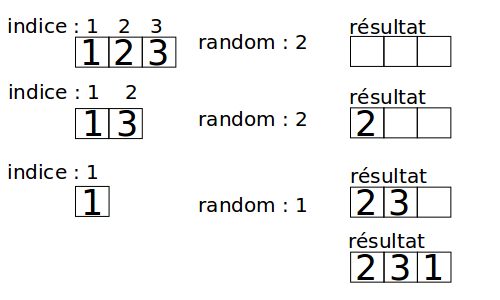
\includegraphics[width=10cm]{tableau_al}\\
		\emph{Ci-dessus, on a à gauche le tableau qui nous sert pour choisir le nombre aléatoire et à droite le tableau que l'on va retourner. A chaque ligne, le nombre tiré aléatoirement représente la case choisie dans le tableau $indice$. On recopie alors le chiffre dans la case dans le tableau $resultat$.\\}
	\end{center}
	
	L'appel de cette fonction pour chaque secteur actif permet de construire un tableau complet avec une affectation de fréquences totalement aléatoire.\\
	Après avoir implémenté cette méthode, il est apparu que la fitness correspondante à la solution aléatoire générée était tout à fait satisfaisante. Il a donc été choisi de la garder.
	
	\section{Optimisation de la solution}
	
	Une fois un première solution trouvée, le travail consiste à l'améliorer du mieux possible. Comme indiqué plus en amont dans ce rapport, l'algorithme d'optimisation choisi est la recherche tabou. Ce choix a été motivé par plusieurs raisons:
	\begin{itemize}
		\item selon les différents documents étudiés sur la recherche tabou, cette méthode paraît appréciée mais surtout suffisamment efficace pour être implémentée dans notre cas;
		\item c'est une méthode assez aisée à comprendre que nous avions vue et qui était donc bien connue de tous les membres du groupe;
		\item les paramètres variables permettent de facilement améliorer l'algorithme jusqu'à trouver un bon équilibre pour une meilleure performance.
	\end{itemize}
	
	L'implémentation de l'algorithme a tout d'abord été rédigé en langage algorithmique, puis traduit en C++. Le code en C++ est disponible en annexe 2 du rapport.\\
	
		\subsection{Algorithme de la méthode}
		
	Au niveau de l'algorithmique, la méthode est assez simple:\\	\begin{lstlisting}
pour NOMBRE_ITERATION faire:

	pour NOMBRE_SITE faire:
	|	sauvegarder la configuration du site
	|
	|	test de la permutation entre secteur 0 et 1
	|	si FITNESS_PERMUTATION < FITNESS_ACTUELLE alors:
	|	|	FITNESS_ACTUELLE = FITNESS_PERMUTATION
	|	|	SITE_ACTUEL = SITE
	|	|	PERMUTATION_SITE_ACTUELLE = NO_PERMUTATION
	|	sinon si FITNESS_PERMUTATION < FITNESS_ACTUELLE_DEGRADEE alors:
	|	|	FITNESS_ACTUELLE_DEGRADEE = FITNESS_PERMUTATION
	|	fsi
	|	
	|	test de la permutation entre secteur 1 et 2
	|	si FITNESS_PERMUTATION < FITNESS_ACTUELLE alors:
	|	|	FITNESS_ACTUELLE = FITNESS_PERMUTATION
	|	|	SITE_ACTUEL = SITE
	|	|	PERMUTATION_SITE_ACTUELLE = NO_PERMUTATION
	|	sinon si FITNESS_PERMUTATION < FITNESS_ACTUELLE_DEGRADEE alors:
	|	|	FITNESS_ACTUELLE_DEGRADEE = FITNESS_PERMUTATION
	|	fsi
	
	|	test de la permutation entre secteur 2 et 0
	|	si FITNESS_PERMUTATION < FITNESS_ACTUELLE alors:
	|	|	FITNESS_ACTUELLE = FITNESS_PERMUTATION
	|	|	SITE_ACTUEL = SITE
	|	|	PERMUTATION_SITE_ACTUELLE = NO_PERMUTATION
	|	sinon si FITNESS_PERMUTATION < FITNESS_ACTUELLE_DEGRADEE alors:
	|	|	FITNESS_ACTUELLE_DEGRADEE = FITNESS_PERMUTATION
	|	fsi
	|   
	|   	retablissement de la configuration sauvegardee du site
	|
	fpour
	
	si FITNESS_ACTUELLE < BEST_FITNESS alors:
	|	BEST_FITNESS = FITNESS_ACTUELLE
	|	BEST_CONF = CONF_ACTUELLE
	|	
	|	effectuer permutation
	|
	|	ajout de la configuration a la liste tabou
	sinon 
	| 	effectuer permutation avec solution degradee
	|
	|	ajout configuration a la liste tabou
	fsi

fpour
		
\end{lstlisting}

\vspace*{1cm}

Pour un nombre d'itérations choisi en paramètre (variant de 5 à 100 dans ce cas), on va tenter de modifier la configuration pour trouver une meilleure fitness.\\
Ainsi, pour chaque site, on sauvegarde tout d'abord la configuration actuelle du site pour pouvoir la restaurer à la fin des tests. Puis, on essaie plusieurs permutations entre les trois secteurs afin de voir s'il y en a une meilleure. Si l'on en trouve une, on remplace la meilleure fitness par celle trouvée. On enregistre alors le site et le type de permutation effectué pour obtenir cette amélioration de fitness.\\
De plus, la recherche tabou devant aussi savoir dégrader une solution s'il n'y en a pas de meilleur pour se sortir d'extremums locaux, ce cas doit \^etre géré. La solution la moins mauvaise est donc toujours enregistrée. Elle est mise à jour avec le numéro du site et le type de permutation. Ainsi, dans le cas où il n'y a pas de meilleure solution, on peut dégrader la solution puisqu'on enregistre un possible changement.\\
Une fois toutes les permutations testée pour un site, on rétablit la configuration d'origine du site et on passe au site suivant.\\
Lorsque tous les sites on été visités, l'algorithme vérifie s'il y a une meilleure solution. S'il en existe une, il la sauvegarde afin d'avoir la meilleure configuration, puis il améliore la solution pour l'itération suivante.\\
 S'il n'en a pas de meilleure, il change seulement la solution pour l'itération suivante.\\
Dans tous les cas, l'algorithme ajoute la solution précédente dans la liste tabou afin de ne pas revenir dessus pendant un certain laps de temps.

			\subsection{Implémentation de la méthode en C++}
			
			Pour l'implémentation informatique de la méthode, il n'a pas suffit de reprendre l'algorithme. En effet, du fait des méthodes existantes du code, toutes les informations ne sont pas disponible comme on le veut. De plus, il faut formaliser les données qui vont être utilisées.\\
			Pour cela, la première chose à considérer est une structure de données, $TabuItem$. Cette structure existait déjà mais a dû être modifiée pour pouvoir fonctionner avec l'algorithme du projet. Cette structure est donc composée :
			\begin{itemize}
				\item d'une configuration;
				\item de la taille de la configuration;
				\item d'une durée tabou restante.
			\end{itemize}
			
			La configuration est en fait un tableau d'entiers qui contient à la suite l'allocation des fréquences de chaque secteur. Cette configuration est bien sûr donnée dans l'ordre. \\
			On peut donc avoir un tableau de la forme:\\ $[f\_site1\_sect1, f_site1\_sect2, f\_site1\_sect3, ...,
 f\_siteN\_sect1, f\_siteN\_sect2, f\_siteN\_sect3]$\\
 avec f signifiant fréquence.\\ \ \\
 
 
 			\paragraph{Les fonctions annexes à $frequencyOptimisation$\\}
 	L'utilisation d'une liste tabou implique que l'on utilise une liste de structures $TabuItem$. L'implémentation implique donc que l'on doit gérer l'ajout d'un $TabuItem$ et la mise à jour de la durée tabou des items de la liste. Une fonction a due être créée pour chacune de ces nécessités.
 	Aussi, l'allocation dynamique des $TabuItem$ et de la liste d'items oblige à la suppression d'un $TabuItem$ en mémoire et la suppression de la liste en mémoire. Deux fonctions ont ainsi été crées.\\ \ \\
 	Un autre problème lors de l'implémentation de l'algorithme est l'accès aux secteurs d'un site. En effet, si la liste des secteurs est disponible, on ne peut récupérer que leur numéro de site au cas par cas. L'inverse, récupérer des secteurs en fonction de leur site, n'est pas possible. Une fonction $find\_secteur\_from\_site$ a donc été implémentée. Cette fonction permet à partir d'un numéro de site de renvoyer les secteurs actifs qui lui sont associés. Cette fonction est primordiale pour l'algorithme puisqu'on a une boucle $pour$ sur les sites.\\ \ \\
	Troisième nécessité pour l'implémentation de l'algorithme: les tests d'égalité. En effet, plusieurs fois dans l'algorithme, il est nécessaire de savoir si deux configurations sont identiques mais aussi si une configuration est présente dans la liste tabou. Ces deux demandes permettent de pouvoir gérer la liste tabou.\\
	Deux fonctions ont été crées, $test\_egal\_conf$ qui permet de savoir si deux configurations sont identiques et $test\_is\_in\_tabu$ qui renvoie un booléen pour savoir si une configuration est dans la liste tabou.\\ \ \\
	Enfin, un dernier problème nécessitant une fonction dédiée est le test de fitness sur une permutation. En effet, pour chaque site, on a à tester des permutations différentes et à calculer l'éventuelle amélioration qu'elle génère. La fonction $test\_permutation$ permet donc, en lui indiquant les deux fréquences de secteurs à échanger, de tester la nouvelle configuration en calculant la nouvelle fitness, puis de remettre la configuration initiale en place et de renvoyer la fitness de la configuration avec permutation.
	
			\paragraph{La fonction $frequencyOptimisation$\\}
			
			Cette fonction implémente peu ou prou l'algorithme qui a été pensé avant le passage informatique. Cependant, les contraintes du programme ont demandé quelques modifications. La plus grosse modification réside dans le fait que l'on ne peut pas récupérer les sites facilement. \\
			Un tableau a donc été mis en place. Ce tableau d'entiers a pour valeur 0 ou 1 dans chaque case. Le tableau est initialisé à 0 au départ et lorsqu'un secteur est testé, le site auquel il appartient et passé à 1 dans le tableau. Cela permet d'effectuer les permutations une seule fois par site, puisque notre boucle se fait sur le nombre de secteur. On évite de nombreux calculs inutiles.
	
	
	

\chapter{Résultats observés}

    \paragraph{}Après avoir terminé la mise en place des algorithmes, nous avons procédé à une
    batterie de tests afin de déterminer le nombre d'itération et la durée de tabou les plus
    efficaces. Nous avons donc exécuté le programme plusieurs fois en alternant le nombre
    d'itération et la durée tabou entre les valeurs 5, 10, 15, 20 et 100.

    \paragraph{}Un fois les tests réalisés, dans on un premier temps on a cherché à définir le
    nombre d'itération le plus intéressant, c'est à dire un nombre suffisamment élevé pour permettre au
    projet de trouver une solution pertinente assez faible pour éviter au programme de tourner trop
    longtemps alors que la meilleur solution locale est obtenue.  
    \begin{center} 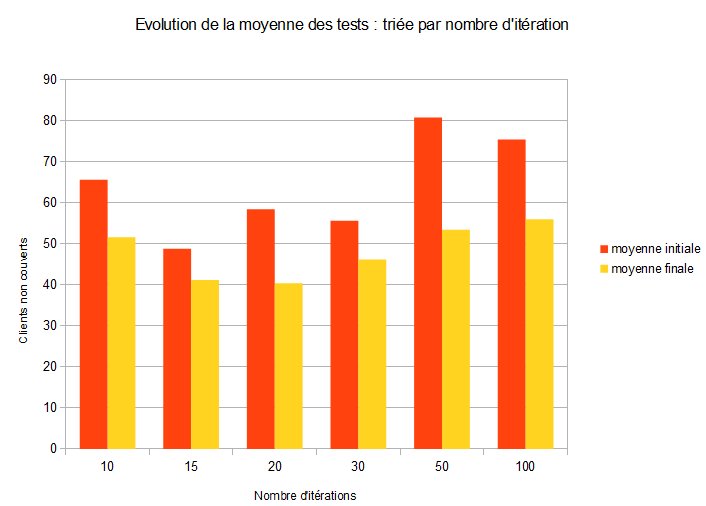
\includegraphics[width=13cm]{tableau_nombre_iteration} \end{center}
    \paragraph{} Suite à nos tests on peut constater que le plus grand écart entre les solutions
    initiales et les solutions finales apparait après 50 itération.

    \paragraph{}Dans un second temps, de la même manière on a cherché à optimisé la valeur de la
    durée tabou, on a donc procédé des tests afin de comparer les différentes valeurs.
    Une bonne durée tabou permet de retirer une solution durant une durée suffisante pour que le
    programme puisse s'éloigner de la solution actuelle pour chercher une nouvelle piste.
    \begin{center} 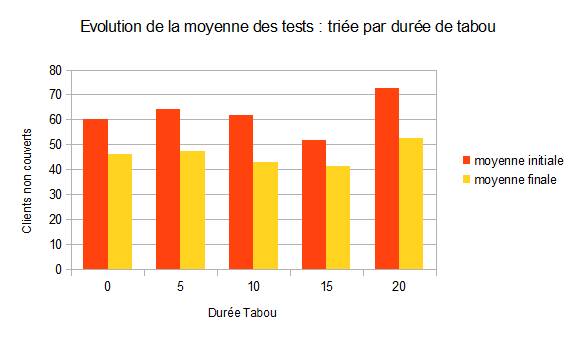
\includegraphics[width=14cm]{tableau_duree_tabou} \end{center}
    \paragraph{}Suite à nos tests on constate que les valeurs les plus pertinentes sont 10 et 20,
    la différence jouant sur le nombre d'itération. Dans l'implémentation de notre solution la durée
    tabou nécessite d'être supérieur à 5 car pour chaque sites 3 permutations sont possible et si
    celle si ne varie pas ou peu l'algorithme restera bloquer sur un site sans visiter les autre
    solution. Une valeur de 10 à 20 permet au programme, dans les cas où les permutations sont
    égales, de visiter des solutions un peu plus éloigné.


    \paragraph{}Ensuite on a réuni nos résultats dans un même graphique afin de représenter les
    meilleurs solutions.
    \begin{center} 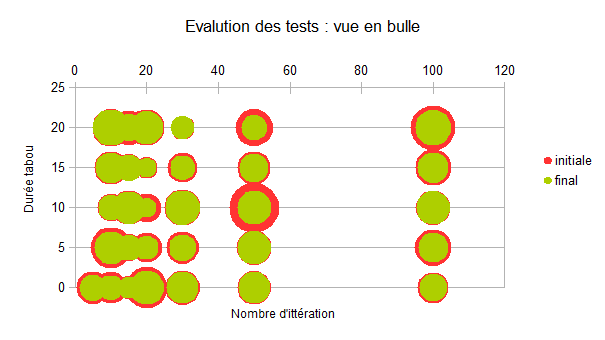
\includegraphics[width=14cm]{tableau_bubulle} \end{center}
    \paragraph{}Le graphique confirme bien les résultats des précédents graphes, la solution avec 50
    itérations et une durée tabou de 10 est la plus efficace.

\chapter{Problèmes rencontrés}

\chapter{Conclusion}
L'algorithme de recherche tabou est fonctionnel. Il permet d'obtenir une fitness très satisfaisante afin d'offrir aux clients la meilleur couverture réseau.

Des améliorations restent possibles en modifiant la méthode du choix des voisins à chaque itération, ou en modifiant la durée de la liste tabou.\\

L'exercice est intéressant car il demande de s'immiscer dans un programme déjà existant, de le comprendre afin d'y ajouter les fonctions à développer. C'est un exercice réaliste puisque dans le monde de l'entreprise, les programmes à développer partent rarement de zéro.\\

Ce projet nous a également permis de nous perfectionner dans le langage C++, de découvrir de nouvelles subtilités et d'améliorer notre manière de programmer. Pour partager les sources du programme, l'utilisation d'un logiciel de gestion de version facilite la tâche.\\

Enfin ce projet a été une expérience enrichissante car effectué au sein d'un groupe de trois étudiants. La communication est importante ainsi que la répartition des tâches. Le travail en groupe permet le partage des compétences et des idées. \\

\appendix
\chapter{Génération de la solution initiale}
\begin{lstlisting}
int* site::randomizeTableFreq(){
    int* tableFreq = new int[3];
    int* table = new int[3]; for(int i=0; i<3;i++)table[i]=i+1;
    int* tableTmp = NULL;
    int taille = 3;
    long random;
    bool shift;
    for(int i=0; i<3; i++)
    {
        shift = false;
        random = Random::aleatoire(taille);
        tableFreq[i]=table[random];
        tableTmp = new int[taille-1];
        for(int j=0; j<taille; j++)
        {
            if(j != random){
                if(shift) tableTmp[j-1] = table[j];
                else tableTmp[j] = table[j];
            }
            else{shift=true;}
        }
        delete table;
        table = tableTmp;
        taille--;
    }
    delete tableTmp;
    return tableFreq;
}
\end{lstlisting}

\chapter{Implémentation de la recherche tabou}
\begin{lstlisting}
/// Implementation de la methode recherche tabou pour l'allocation des frequences
// Liste des sites voisins du site choisi
//Le liste tabou contenant le meilleur site voisins et la duree qui lui correspond
struct TabuItem{
    TabuItem():conf(NULL),dureeTabu(0){}
    int* conf;
    int conf_taille;
    int dureeTabu;
};

void add_Item_ListeTabuItems(ListeTabuItems* liste,int* conf, int dureeTabu){
    if(liste->nbItems == 0){
        liste->ListeItems = new TabuItem*[1];
        liste->nbItems = 1;
    }
    else{
        TabuItem** tmpListe = new TabuItem*[liste->nbItems + 1];
        for(int i=0; i<liste->nbItems; i++)
            tmpListe[i] = liste->ListeItems[i];
        liste->nbItems++;
        delete liste->ListeItems;
        liste->ListeItems = tmpListe;
    }
    TabuItem* item = new TabuItem();
    item->conf = conf;
    item->dureeTabu = dureeTabu;
    liste->ListeItems[liste->nbItems - 1] = item;
}

void update_Items_ListeTabuItems(ListeTabuItems* liste){
    int new_nbItems=0;
    for(int i=0; i<liste->nbItems;i++){
        if(liste->ListeItems[i]->dureeTabu != 0) new_nbItems ++;
    }
    TabuItem** tmpListe = new TabuItem*[new_nbItems];
    TabuItem* item = NULL;
    int index=0;
    for(int i=0; i<liste->nbItems;i++){
        if(liste->ListeItems[i]->dureeTabu != 0){
            item = new TabuItem();
            item->conf = liste->ListeItems[i]->conf;
            item->dureeTabu = liste->ListeItems[i]->dureeTabu - 1;
            tmpListe[index] = item;
            index++;
        }
    }
    liste->nbItems = new_nbItems;
    delete liste->ListeItems;
    liste->ListeItems = tmpListe;
}

void delete_item(TabuItem* item){
    delete item->conf;
    delete item;
}

void delete_ListeTabuItems(ListeTabuItems* liste){
    for(int i=0; i<liste->nbItems;i++)
        delete_item(liste->ListeItems[i]);
    delete liste;
}

void find_secteur_from_site(int no_site,secteur** lesSecteurA, int nb_secteur_a,secteur** &secteurs)
{
    int index_secteur = 0;

    for(int i=0; i<nb_secteur_a;i++)
    {
        if(index_secteur == 3)break;

        if(lesSecteurA[i]->get_site()->get_no() == no_site)
        {
            secteurs[index_secteur] = lesSecteurA[i];
            index_secteur++;
        }
    }
    for(index_secteur; index_secteur<3; index_secteur++)
            secteurs[index_secteur]= NULL;
}

bool test_egal_conf(int* conf1,int* conf2, int nb_secteur_a)
{
    for(int i=0; i<nb_secteur_a;i++)
        if(conf1[i] != conf2[i])
            return false;
    return true;
}

bool test_is_in_tabu(int* &conf,int nb_secteur_a,ListeTabuItems* &listeTabu)
{
    for(int i=0; i<listeTabu->nbItems;i++)
    {
        if(test_egal_conf(conf,listeTabu->ListeItems[i]->conf,nb_secteur_a))
            return true;
    }
    return false;
}

double test_permutation(int stable,pointTest** lesPTA,int nb_tp_a,
                        secteur** &lesSecteurA,int nb_secteur_a,int no_scen,
                        ListeTabuItems* &listeTabu,
                        secteur** &secteurs,int index1,int index2)
{

    //return 99999 : pour dire que c'est une enorme fitness

    if(secteurs[index1] == NULL || secteurs[index2] == NULL)
        return 9999;

    int porteuse;

    porteuse = secteurs[index1]->get_porteuse();
    secteurs[index1]->set_porteuse(secteurs[index2]->get_porteuse());
    secteurs[index2]->set_porteuse(porteuse);

    int* conf = new int[nb_secteur_a];
    for(int i = 0; i < nb_secteur_a; i++){
        conf[i] = lesSecteurA[i]->get_porteuse();
    }
    double result = 9999;
    if(test_is_in_tabu(conf,nb_secteur_a,listeTabu) == false)
       result = Fitness::eval(stable,lesPTA, nb_tp_a, lesSecteurA, nb_secteur_a, no_scen);
    delete conf;


    porteuse = secteurs[index1]->get_porteuse();
    secteurs[index1]->set_porteuse(secteurs[index2]->get_porteuse());
    secteurs[index2]->set_porteuse(porteuse);

    return result;
}

///Implementez votre methode ici
/** nom = nom du fichier de sortie
*   stable = on y touche pas. variable de stabilisation de l'affectation d'une
*   antenne a un point test
*   lesPTA = liste de tous les pts test actifs (actif = au moins un client dans le point test
*   nb_tp_a = nombre de pts test actifs
*   lesSecteurA = lste des secteurs comportant au moins un point test actif
*   nb_secteur_a = nombre de secteurs actifs
*   no_scen = le numero du scenario on n'y touche pas.
*/
void optimisation::frequencyOptimization(char *nom, int stable, pointTest** lesPTA, int nb_tp_a, secteur** lesSecteurA, int nb_secteur_a, int no_scen){

	//USE main.cpp l. 160
    // UTILE secteur::getporteuse() et secteur::getsite()

    cout<<endl<<endl<<endl<<endl;
    cout<<"--------------------------"<<endl<<endl;
    cout<<"Parametre de la fonction : "<<endl<<endl;

    cout<<"nom : "<<nom<<endl;
    cout<<"stable : "<<stable<<endl;
    cout<<"nb_tp_a : "<<nb_tp_a<<endl;
    cout<<"nb_secteur_a : "<<nb_secteur_a<<endl;
    cout<<"no_scen : "<<no_scen<<endl;

    GOutputFile file_sortie(nom);
	file_sortie.open();
    file_sortie << "Optimisation robuste des frequences" << "\n";
    file_sortie << "les parametres de l'optimisation" << "\n";
    file_sortie <<"12h15"<< "\n";
    file_sortie << "facteur de stabilite= " << stable << "\n";
    file_sortie << "le critere est le nombre de clients non couverts"<< "\n";
	double nb_clients_non_couvert = 0.0;
	double best_nb_clients_non_couvert = Fitness::eval(stable,lesPTA, nb_tp_a, lesSecteurA, nb_secteur_a, no_scen);
	double best_nb_clients_non_couvert2 = best_nb_clients_non_couvert+1;
    cout<<endl<<"--------------------------"<<endl;



    ListeTabuItems* listeTabu = new ListeTabuItems();
    Table_sites* voisin = NULL;
    double NB_CLIENT= 3846;
    int NB_ITERATION = 100;
    int DUREE_TABU = 20;

    int* BEST_CONF = new int[nb_secteur_a];
    for(int i = 0; i < nb_secteur_a; i++){BEST_CONF[i] = lesSecteurA[i]->get_porteuse();}
    int INIT_FITNESS = best_nb_clients_non_couvert;
    int BEST_FITNESS = best_nb_clients_non_couvert;

    int ITERATE_SITE = -1;     // pas de changement
    int ITERATE_PERM = 0;     // pas de permutation
    double ITERATE_FITNESS = 9999;

    int BOF_SITE = -1;
    int BOF_PERM = -1 ;
    double BOF_FITNESS = 9999;


    int tmp=-1;
    int nb_site_a=0;
    for(int i=0; i<nb_secteur_a;i++)
    {
        if(lesSecteurA[i]->get_site()->get_no() != tmp)
        {
            nb_site_a++;
            tmp = lesSecteurA[i]->get_site()->get_no();
        }
    }

    int* sites_visites = new int[nb_secteur_a/3];
    int no_site = -1;
    int* etat_site = new int[3];
    secteur** secteurs = new secteur*[3];
    int porteuse;
    double fitness_tmp;
    int index1,index2;
    int* conf =NULL;
    double init_fitness = 0;

    cout << "Fitness initiale: " << best_nb_clients_non_couvert <<"   "<<best_nb_clients_non_couvert/NB_CLIENT*100<<"%  "<<endl;

    for(int iteration=0; iteration<NB_ITERATION;iteration++ )
    {
        //On nettoie la liste des passages
        for( int site=0; site < nb_secteur_a/3; site++)sites_visites[site] = 0;
        ITERATE_SITE = -1;ITERATE_PERM = -1;
        BOF_SITE = -1;BOF_PERM = -1;BOF_FITNESS = 9999;


        //Pour chaque secteur
        int no_secteur=0;
        init_fitness = ITERATE_FITNESS;

        for(no_secteur; no_secteur<nb_secteur_a; no_secteur++)
        {
            no_site = lesSecteurA[no_secteur]->get_site()->get_no();
            //Si le site n'as pas encore ete visite
            if(sites_visites[no_site] == 0)
            {
                //on recupere les secteurs du site
                find_secteur_from_site(no_site,lesSecteurA,nb_secteur_a,secteurs);
                //On recupere l'etat du site
                for(int i=0;i<3;i++)
                {
                    if(secteurs[i] == NULL) etat_site[i] = -1;
                    else etat_site[i] = secteurs[i]->get_porteuse();
                }



                //ESSAI permutation (1)       secteurs[0] <-> secteurs[1]
                fitness_tmp = test_permutation(stable,lesPTA, nb_tp_a, lesSecteurA, nb_secteur_a, no_scen,listeTabu,secteurs,0,1);
                if(fitness_tmp < ITERATE_FITNESS)
                {ITERATE_FITNESS = fitness_tmp; ITERATE_SITE = no_site; ITERATE_PERM = 1;}
                else if(fitness_tmp != 9999 && init_fitness< fitness_tmp && fitness_tmp <= BOF_FITNESS)
                {BOF_FITNESS = fitness_tmp; BOF_SITE = no_site; BOF_PERM = 1;}
                //ESSAI permutation (2)       secteurs[1] <-> secteurs[2]
                fitness_tmp = test_permutation(stable,lesPTA, nb_tp_a, lesSecteurA, nb_secteur_a, no_scen,listeTabu,secteurs,1,2);
                if(fitness_tmp < ITERATE_FITNESS)
                {ITERATE_FITNESS = fitness_tmp; ITERATE_SITE = no_site; ITERATE_PERM = 2;}
                else if(fitness_tmp != 9999 && init_fitness< fitness_tmp && fitness_tmp <= BOF_FITNESS)
                {BOF_FITNESS = fitness_tmp; BOF_SITE = no_site; BOF_PERM = 2;}
                //ESSAI permutation (3)       secteurs[0] <-> secteurs[2]
                fitness_tmp = test_permutation(stable,lesPTA, nb_tp_a, lesSecteurA, nb_secteur_a, no_scen,listeTabu,secteurs,0,2);
                if(fitness_tmp < ITERATE_FITNESS)
                {ITERATE_FITNESS = fitness_tmp; ITERATE_SITE = no_site; ITERATE_PERM = 3;}
                else if(fitness_tmp != 9999 && init_fitness< fitness_tmp && fitness_tmp <= BOF_FITNESS)
                {BOF_FITNESS = fitness_tmp; BOF_SITE = no_site; BOF_PERM = 3;}


                //On retablit les valeurs d'origine du site
                for(int i=0;i<3;i++)
                {
                    if(secteurs[i] != NULL)
                    {secteurs[i]->set_porteuse(etat_site[i]);}
                }

                sites_visites[no_site] = 1;
            }
        }


        update_Items_ListeTabuItems(listeTabu);


        //Si on a trouver une meilleur permutation on la fait
        if(ITERATE_PERM == -1)
        {
            ITERATE_FITNESS = BOF_FITNESS;
            ITERATE_PERM = BOF_PERM;
            ITERATE_SITE = BOF_SITE;
        }

        if(ITERATE_FITNESS < BEST_FITNESS)
        {
            for(int i = 0; i < nb_secteur_a; i++){BEST_CONF[i] = lesSecteurA[i]->get_porteuse();}
            BEST_FITNESS = ITERATE_FITNESS;
            cout << "Fitness tour  "<<iteration<<"  :  "<< BEST_FITNESS <<"   "<<BEST_FITNESS/NB_CLIENT*100<<"%  "<< endl;
        }

        find_secteur_from_site(ITERATE_SITE,lesSecteurA,nb_secteur_a,secteurs);
         switch(ITERATE_PERM){
             case 1 : index1=0;index2=1; break;
             case 2 : index1=1;index2=2; break;
             case 3 : index1=0;index2=2; break;
         }


        porteuse = secteurs[index1]->get_porteuse();
        secteurs[index1]->set_porteuse(secteurs[index2]->get_porteuse());
        secteurs[index2]->set_porteuse(porteuse);


        conf = new int[nb_secteur_a];
        for(int i = 0; i < nb_secteur_a; i++){conf[i] = lesSecteurA[i]->get_porteuse();}

        add_Item_ListeTabuItems(listeTabu,conf,DUREE_TABU);

    }

    delete secteurs;
    delete etat_site;
    delete sites_visites;
    delete_ListeTabuItems(listeTabu);


    cout<<endl<<"--------------------------"<<endl;
    cout<<endl<<endl<<endl<<endl;

    file_sortie.close();

}
\end{lstlisting}

\end{document}
